\documentclass[conference]{IEEEtran}
\IEEEoverridecommandlockouts
% The preceding line is only needed to identify funding in the first footnote. If that is unneeded, please comment it out.
\usepackage{cite}
\usepackage{bm}
\usepackage{amsmath,amssymb,amsfonts}
\usepackage{algorithmic}
\usepackage{graphicx}
\usepackage{textcomp}
\usepackage{xcolor}
\def\BibTeX{{\rm B\kern-.05em{\sc i\kern-.025em b}\kern-.08em
    T\kern-.1667em\lower.7ex\hbox{E}\kern-.125emX}}
\begin{document}

\title{Dynamic I/O Model Recommendation System With Machine Learning\\
{\footnotesize \textsuperscript{*}Note: Sub-titles are not captured in Xplore and
should not be used}
\thanks{Identify applicable funding agency here. If none, delete this.}
}

\author{\IEEEauthorblockN{1\textsuperscript{st} Given Name Surname}
    \IEEEauthorblockA{\textit{dept. name of organization (of Aff.)} \\
        \textit{name of organization (of Aff.)}\\
        City, Country \\
        email address or ORCID}
    \and
    \IEEEauthorblockN{2\textsuperscript{nd} Given Name Surname}
    \IEEEauthorblockA{\textit{dept. name of organization (of Aff.)} \\
        \textit{name of organization (of Aff.)}\\
        City, Country \\
        email address or ORCID}
}

\maketitle

\begin{abstract}
    In a typical database and file system, using asynchronous I/O is generally a good way to optimize processing efficiency.
    However, each process and application mainly focus on its own performance, rarely consider the global performance of the system.
    In this work, in order to balance the I/O performance and resources in a system, we use Machine Learning(ML) techniques to learn I/O model's performance, 
    and set up a client/server system based on gRPC to recommend the more efficient I/O model under different system loads. Which is high performance, scalable, cross-platform and easy to adapt.
    The experimental result shows that our system has a 15\% performance improvement compared to using asynchronous I/O alone and only cost little system resources.

\end{abstract}

\renewcommand\IEEEkeywordsname{Keywords}
\begin{IEEEkeywords}
    asynchronous I/O, synchronous I/O, Machine Learning, performance prediction, gRPC 
\end{IEEEkeywords}

\section{Introduction}

% \begin{itemize}
%     \item Data center is popular and I/O is one of the bottlenecks
%     \item asynchronous and synchronous I/O
%     \item Machine Learning
%     \item structure of my system
% \end{itemize}
    
With revolution of “Big Data” and “Cloud Computing”, data center has expended to a large scale and data has grown exponentially. 
Therefore, data center has to process hundreds of millions of pictures and hundreds of billions of messages each day.
How to improve processing efficiency is a hot issue of a data center. 
Due to the huge speed gap between CPU and I/O device, I/O is one of the bottlenecks of the issue.
Using asynchronous I/O is a common way to boost I/O speed. Synchronous and asynchronous I/O are two types of I/O synchronizations as  \emph{\textbf{\large{figure 1}}} shows. 
In a synchronous I/O job, it starts a thread for I/O operation, and it would hang immediately until the operation is finished.
While in an asynchronous I/O job, it would start a thread to send a I/O request to Kernel by calling a function, if the request is accepted successfully, it continues to process other jobs. 
The kernel signals the calling thread when the operation is finished, then the thread interrupts its current job and processes the data from the I/O operation as soon as possible.
However, using asynchronous I/O frequently requires much CPU resources and the I/O's latency would become higher when the I/O's depth is longer.

\begin{figure}[htbp]
        \centering
        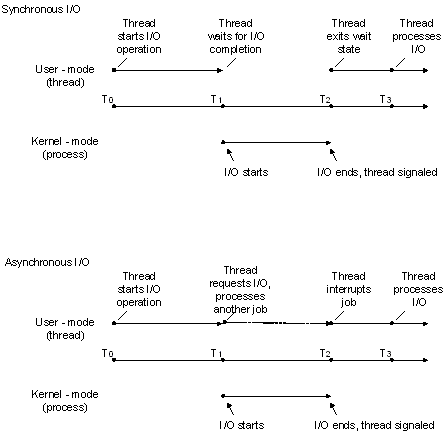
\includegraphics[width=0.45\textwidth]{fig2bedit.png}
        \caption{Asynchronous and Synchronous I/O}
        % \label{fig}
\end{figure}

To help improve system I/O and processing efficiency, we purpose to combine I/O with Machine Learning(ML). The I/O synchronizations of each I/O's engine 
have different performance when it is facing different kinds of I/O job and different system load. Collecting these I/O data and training into a Decision Tree model 
which can predict the most suitable I/O method in current situation. And setting up a Client/Server-based recommendation system using gRPC framework to decide using which kind of I/O for each I/O job.


The main challenge of our system is performance, since each I/O job have to call the server for the better I/O method which cost much time on process communication and prediction.
To solve the related problems, we use memory cache and gRPC framework. The data is serialized to protocol buffers and passed by stream, meanwhile, store the hot data into cache.
Therefore, the communication's time will be shortened and reuse the prediction result. After the improvements applied in our system, Running the same task has an efficiency increase of nearly 15\%.

In summary, we have made the following contributions in our paper:
\begin{enumerate}
    \item Train a Decision Tree model which can predict the best I/O method base on the current system load.
    \item We build a Client/Server-based, lightweight and scalable system using gRPC to help each I/O job improve efficiency.
    \item Run a script to make the system self-optimization daily.
\end{enumerate}

The rest of the paper is organized as follow.





\section{Design}
In this section we talk about the goals of our system first and then show the overview architecture.
\subsection{Goals}
\begin{itemize}
    \item High-performance.
    \item Scalable.
    \item Self-optimization.
\end{itemize}

\subsection{Overview}
figure.

\subsection{Techniques}

\begin{itemize}
    \item Machine Learning
    \item Decision Tree
    \item gRPC
    \item atomic
    \item redis 
\end{itemize}


% \begin{itemize}
%     \item evaluate io-uring performance and compare to other ioengins and synchronous
%     \item why choosing machine learning and decision-tree
%     \item how to connect client and server
% \end{itemize}


% \subsection{Maintaining the Integrity of the Specifications}


\section{Implementation}
\begin{itemize}
    \item collect data
    \item train data
    \item build the system
    \item test the system
\end{itemize}

% \subsection{Abbreviations and Acronyms}\label{AA}

% \subsection{Units}
% \begin{itemize}
%     \item Use 
%     \item Avoid.
%     \item Do 
%     \item Use 
% \end{itemize}

% \subsection{Equations}
% \begin{equation}
%     a+b=\gamma\label{eq}
% \end{equation}

% \subsection{Figures and Tables}
% \paragraph{Positioning Figures and Tables} Place figures and tables at the top and

% \begin{table}[htbp]
%     \caption{Table Type Styles}
%     \begin{center}
%         \begin{tabular}{|c|c|c|c|}
%             \hline
%             \textbf{Table} & \multicolumn{3}{|c|}{\textbf{Table Column Head}}                                                         \\
%             \cline{2-4}
%             \textbf{Head}  & \textbf{\textit{Table column subhead}}           & \textbf{\textit{Subhead}} & \textbf{\textit{Subhead}} \\
%             \hline
%             copy           & More table copy$^{\mathrm{a}}$                   &                           &                           \\
%             \hline
%             \multicolumn{4}{l}{$^{\mathrm{a}}$Sample of a Table footnote.}
%         \end{tabular}
%         \label{tab1}
%     \end{center}
% \end{table}

% \begin{figure}[htbp]
%     \centerline{
\includegraphics{fig1.png}}
%     \caption{Example of a figure caption.}
%     \label{fig}
% \end{figure}


\section{Evaluation}
\begin{itemize}
    \item io-uring performance
    \item compare single I/O work performance between used and none-used our system 
    \item compare multi I/O works performance between used and none-used our system 
\end{itemize}

\section{Related Work}
\begin{itemize}
    \item hot issue in I/O
\end{itemize}

\section{Conclusion}
    improvement of our system and future usage scenario

\section*{Acknowledgment}


% \section*{References}


\begin{thebibliography}{00}
    \bibitem{b1} G. Eason, B. Noble, and I. N. Sneddon, ``On certain integrals of Lipschitz-Hankel type involving products of Bessel functions,'' Phil. Trans. Roy. Soc. London, vol. A247, pp. 529--551, April 1955.
\end{thebibliography}
\vspace{12pt}
\color{red}
IEEE conference templates contain guidance text for composing and formatting conference papers. Please ensure that all template text is removed from your conference paper prior to submission to the conference. Failure to remove the template text from your paper may result in your paper not being published.

\end{document}
